%%% !Mode\dots "XeLaTeX:UTF-8"
%%% author : liuzheng712@gmail.com(刘正)
\documentclass[a4paper,12pt]{article}
%%% !Mode\dots "XeLaTeX:UTF-8"

\XeTeXlinebreaklocale ``zh''
\XeTeXlinebreakskip = 0pt plus 1pt minus 0.1pt
\usepackage{fontspec,xunicode,xltxtra}
\usepackage{titlesec}			% 自定义章节标题包
\usepackage{titletoc}			% 自定义章节目录包
\usepackage{hyperref}			% 超链接
%\usepackage[colorlinks,linkcolor=black,anchorcolor=black,citecolor=black]{hyperref}	% 超链接如果不想要红框的话,打印时是不会打出框的
\usepackage{color}              % 彩色
\usepackage{xcolor}             % 彩色
\usepackage{listings}           % 代码风格
\usepackage{courier}
\usepackage[boldfont]{xeCJK}				% CJK字体宏包
\usepackage{xCJKnumb}
%\usepackage{times}
\setmainfont{Times New Roman}
\setsansfont{Times New Roman}
\setmonofont{Times New Roman}
\setCJKmainfont[BoldFont=SimHei]{SimSun}
%\setCJKmainfont{Adobe Song Std} 	% 设定中文为宋体
%\usepackage{CJKutf8}                % 中文
\usepackage{graphicx}           % 图片
\usepackage{subfigure}
\usepackage{geometry}           % 页面设置

\usepackage{indentfirst}        % 首行缩进
\setlength{\parindent}{2em}     % 首行缩进2字符
\usepackage{amstext}            % 使公式中使用text标签现实中文
\usepackage{fancyhdr}           % 页眉页脚
\usepackage{ulem}				% 下划线
\usepackage{pdfpages}           % 用于嵌入pdf
\usepackage{multirow}           %使用多栏宏包
\usepackage{longtable}
\usepackage{amsmath}
\usepackage{multicol}
\usepackage{amssymb}
\usepackage{float}				% 表格固定
\usepackage{latexsym}			% 获得特殊数学二元运算符
\usepackage[justification=centering]{caption}
\usepackage{enumerate}
\usepackage{animate}

% 页眉设置
\geometry{left=2.5cm,right=2.5cm,bottom=2.5cm,top=3cm}

\begin{document}
%%% !Mode\dots "XeLaTeX:UTF-8"

\pagenumbering{arabic}          % 页码数字
\setcounter{page}{1}            % 页码起始数字
\renewcommand{\sfdefault}{phv}
\definecolor{dkgreen}{rgb}{0,0.6,0}
\definecolor{gray}{rgb}{0.5,0.5,0.5}

% 行距 1.25
\renewcommand{\baselinestretch}{1.25}
\newcommand{\tablecell}[2]{\begin{tabular}{@{}#1@{}}#2\end{tabular}}   % 表格内换行,用法\tablecell{c}{balabalba\\balabalba}
\graphicspath{{figures/}}  		% 图路径 

%%%%%%字体部分%%%%%%%%
\newfontfamily\fangsong{FangSong}     % 仿宋
\newfontfamily\hei{SimHei}             % 黑体
\newfontfamily\kai{KaiTi}             % 楷体
\newfontfamily\song{SimSun}             % 宋体
\newfontfamily\lishu{LiSu}             			% 隶书
\newfontfamily\yahei{Microsoft YaHei}          	% 微软雅黑
\newfontfamily\times{Times New Roman}
%\newfontfamily\monaco{Monaco}

%%%%%%%字号%%%%%%%
%%%%%%单倍%%%%%%%%
\newcommand{\yihao}{\fontsize{26pt}{26pt}\selectfont}       % 一号, 单倍行距
\newcommand{\xiaoyi}{\fontsize{24pt}{24pt}\selectfont}      % 小一, 单倍行距
\newcommand{\erhao}{\fontsize{22pt}{22pt}\selectfont}       % 二号, 单倍行距
\newcommand{\xiaoer}{\fontsize{18pt}{18pt}\selectfont}      % 小二, 单倍行距
\newcommand{\sanhao}{\fontsize{16pt}{16pt}\selectfont}      % 三号, 单倍行距
\newcommand{\xiaosan}{\fontsize{15pt}{15pt}\selectfont}     % 小三, 单倍行距
\newcommand{\sihao}{\fontsize{14pt}{14pt}\selectfont}       % 四号, 单倍行距
\newcommand{\xiaosi}{\fontsize{12pt}{12pt}\selectfont}      % 小四, 单倍行距
\newcommand{\wuhao}{\fontsize{10.5pt}{10.5pt}\selectfont}   % 五号, 单倍行距
\newcommand{\xiaowu}{\fontsize{9pt}{9pt}\selectfont}        % 小五, 单倍行距

%%%%%%1.5倍%%%%%%%
\newcommand{\Yihao}{\fontsize{26pt}{39pt}\selectfont}       % 一号, 1.5倍行距
\newcommand{\Xiaoyi}{\fontsize{24pt}{36pt}\selectfont}      % 小一, 1.5倍行距
\newcommand{\Erhao}{\fontsize{22pt}{33pt}\selectfont}       % 二号, 1.5倍行距
\newcommand{\Xiaoer}{\fontsize{18pt}{27pt}\selectfont}      % 小二, 1.5倍行距
\newcommand{\Sanhao}{\fontsize{16pt}{24pt}\selectfont}      % 三号, 1.5倍行距
\newcommand{\Xiaosan}{\fontsize{15pt}{22.5pt}\selectfont}   % 小三, 1.5倍行距
\newcommand{\Sihao}{\fontsize{14pt}{21pt}\selectfont}       % 四号, 1.5倍行距
\newcommand{\Xiaosi}{\fontsize{12pt}{18pt}\selectfont}      % 小四, 1.5倍行距
\newcommand{\XIaosi}{\fontsize{12pt}{15pt}\selectfont}      % 小四, 1.25倍行距
\newcommand{\Wuhao}{\fontsize{10.5pt}{15.75pt}\selectfont}  % 五号, 1.5倍行距
\newcommand{\Xiaowu}{\fontsize{9pt}{13.5pt}\selectfont}     % 小五, 1.5倍行距

%%%%%%%%%% Table, Figure and Equation %%%%%%%%%%%%%%%%%
%\renewcommand{\thefigure}{\arabic{section}-\arabic{figure}}       % 使图编号为 7-1 的格式 
%\renewcommand{\thesubfigure}{\alph{subfigure})}                   % 使子图编号为 a) 的格式
%\renewcommand{\thesubtable}{(\alph{subtable})}                    % 使子表编号为 (a) 的格式
%\renewcommand{\thetable}{\arabic{section}-\arabic{table}}         % 使表编号为 7-1 的格式
%\renewcommand{\theequation}{\arabic{section}-\arabic{equation}}   % 使公式编号为 7-1 的格式

%%%%%%%%%% Chapter and Section %%%%%%%%%%%%%
\setlength{\parindent}{2em}
\def\cnarticle
{

\newcommand{\shijian}{\number\year~年~\number\month~月~\number\day~日}
\renewcommand{\tablename}{\song\wuhao 表}                                     % 插表题头
\renewcommand{\figurename}{\song\wuhao 图}                                    % 插图题头

\titleformat{\section}{\sihao\hei\bfseries}{\hei\thesection}{1em}{}
\titlespacing{\section}{0pt}{\baselineskip}{0.3\baselineskip}

\titleformat{\subsection}{\sihao\hei\bfseries}{\hei\thesubsection}{1em}{}
\titlespacing{\subsection}{0pt}{0.1\baselineskip}{0.3\baselineskip}

\titleformat{\subsubsection}{\sihao\hei}{\thesubsubsection}{1em}{}
\titlespacing{\subsubsection}{0pt}{0.05\baselineskip}{0.1\baselineskip}

\renewcommand{\refname}{参考文献}
}
%

%%%%%%%%%%%%%%%%%%%%%%%% Code %%%%%%%%%%%%%%%%%%%%%%%%%
\lstset{
        language=matlab,            % 设定默认语言为MATLAB
        keywords={break,case,catch,continue,else,elseif,end,for,function,
        global,if,otherwise,persistent,return,switch,try,while}, %设定关键词列表
        keywordstyle=\color{blue},  % 关键词为蓝色
        commentstyle=\color{dkgreen},       % 注释为绿色
        stringstyle=\color{red},    % 字符串为红色
        %basicstyle=\xiaosi\monaco, % 基本字体的字号
        basicstyle=\xiaosi\times, % 基本字体的字号
        breaklines=true,            % 自动将长代码行换行排版
        breakatwhitespace=true,     % 断行只在空格处
        extendedchars=false,        % 解决代码跨页时,章节标题页眉等汉字不显示问题
        showspaces=false,           % 不显示空格
        showstringspaces=true,      % 字符串中显示空格
        showtabs=false,             % 不显示TAB键
        tabsize=4,                  % TAB被当成4个空格
        frame=l,                    % 显示边框
        numbers=left,               % 显示行号
        numberstyle=\tiny,          % 行号字体为tiny
        numbersep=9pt,              % 行号垂直位置
        numberstyle=\normalsize,  % 行号字体的字号
        stepnumber=1,               % 行号显示的步长
        keywordstyle=\color{blue}\bfseries, % 特殊代码高亮蓝色加粗
        backgroundcolor=\color{white},      % 背景色 需要 \usepackage{color}
        escapeinside={/*@}{@*/}     % 添加注释,暂时离开
        }
\renewcommand{\lstlistingname}{CODE}
\lstloadlanguages{% Check Dokumentation for further languages ...
        MATLAB
}

\pagestyle{fancy}
\fancypagestyle{plain}

\def\yemeiclean
{
	\fancyhead{}                        % 清空页眉
	\renewcommand{\headrulewidth}{0pt}       %把页眉线的宽度设为零,即去掉页眉线	
}


\newcommand{\cankao}[1]{$^{\mbox{\protect \scriptsize \cite{#1}}}$}% 修改引用文件样式
\newcommand{\tabincell}[2]{\begin{tabular}{@{}#1@{}}#2\end{tabular}}

\cnarticle			% 中文论文环境,默认是英文的
%\renewcommand{\thefigure}{\arabic{section}-\arabic{figure}}       % 使图编号为 7-1 的格式 
%\renewcommand{\thesubfigure}{\alph{subfigure})}                   % 使子图编号为 a) 的格式
%\renewcommand{\thesubtable}{(\alph{subtable})}                    % 使子表编号为 (a) 的格式
%\renewcommand{\thetable}{\arabic{section}-\arabic{table}}         % 使表编号为 7-1 的格式
%\renewcommand{\theequation}{\arabic{section}-\arabic{equation}}   % 使公式编号为 7-1 的格式
\yemeiclean  % 清理页眉,注释掉会显示页眉

\begin{center}
\sihao   支持向量机通俗导论(理解SVM的三层境界)
\wuhao

作者:July、pluskid ;致谢:白石、JerryLead

出处:结构之法算法之道blog。

\end{center}
%\begin{multicols}{2}
\section*{前言}
动笔写这个支持向量机(support vector machine)是费了不少劲和困难的,原因很简单,一者这个东西本身就并不好懂,要深入学习和研究下去需花费不少时间和精力,二者这个东西也不好讲清楚,尽管网上已经有朋友写得不错了(见文末参考链接),但在描述数学公式的时候还是显得不够。得益于同学白石的数学证明,我还是想尝试写一下,希望本文在兼顾通俗易懂的基础上,真真正正能足以成为一篇完整概括和介绍支持向量机的导论性的文章。

本文在写的过程中,参考了不少资料,包括《支持向量机导论》、《统计学习方法》及网友pluskid的支持向量机系列等等,于此,还是一篇学习笔记,只是加入了自己的理解和总结,有任何不妥之处,还望海涵。全文宏观上整体认识支持向量机的概念和用处,微观上深究部分定理的来龙去脉,证明及原理细节,力保逻辑清晰 \& 通俗易懂。

同时,阅读本文时建议大家尽量使用chrome等浏览器,如此公式才能更好的显示,再者,阅读时可拿张纸和笔出来,把本文所有定理.公式都亲自推导一遍或者直接打印下来(可直接打印网页版或本文文末附的PDF,享受随时随地思考、演算的极致快感),在文稿上演算。

Ok,还是那句原话,有任何问题,欢迎任何人随时不吝指正 \& 赐教,感谢。

\section{第一层、了解SVM}
\subsection{什么是支持向量机SVM}
要明白什么是SVM,便得从分类说起。

分类作为数据挖掘领域中一项非常重要的任务,它的目的是学会一个分类函数或分类模型(或者叫做分类器),而支持向量机本身便是一种监督式学习的方法(至于具体什么是监督学习与非监督学习,请参见此系列Machine L\&Data Mining第一篇),它广泛的应用于统计分类以及回归分析中。

支持向量机(SVM)是90年代中期发展起来的基于统计学习理论的一种机器学习方法,通过寻求结构化风险最小来提高学习机泛化能力,实现经验风险和置信范围的最小化,从而达到在统计样本量较少的情况下,亦能获得良好统计规律的目的。

通俗来讲,它是一种二类分类模型,其基本模型定义为特征空间上的间隔最大的线性分类器,即支持向量机的学习策略便是间隔最大化,最终可转化为一个凸二次规划问题的求解。

对于不想深究SVM原理的同学或比如就只想看看SVM是干嘛的,那么,了解到这里便足够了,不需上层。而对于那些喜欢深入研究一个东西的同学,甚至究其本质的,咱们则还有很长的一段路要走,万里长征,咱们开始迈第一步吧,相信你能走完。

\subsection{线性分类}
OK,在讲SVM之前,咱们必须先弄清楚一个概念:线性分类器(也可以叫做感知机,这里的机表示的是一种算法,本文第三部分、证明SVM中会详细阐述)。

\subsubsection{分类标准}
  这里我们考虑的是一个两类的分类问题,数据点用 $ x $ 来表示,这是一个 $ n $ 维向量,$ w^T $中的$ T $代表转置,而类别用 $ y $ 来表示,可以取 1 或者 -1 ,分别代表两个不同的类。一个线性分类器的学习目标就是要在 $ n $ 维的数据空间中找到一个分类超平面,其方程可以表示为:

\begin{equation}
w^Tx+b=0
\end{equation}

上面给出了线性分类的定义描述,但或许读者没有想过:为何用y取1 或者 -1来表示两个不同的类别呢?其实,这个1或-1的分类标准起源于logistic回归,为了完整和过渡的自然性,咱们就再来看看这个logistic回归。

\subsubsection{1或-1分类标准的起源:logistic回归}
Logistic回归目的是从特征学习出一个$0/1$分类模型,而这个模型是将特性的线性组合作为自变量,由于自变量的取值范围是负无穷到正无穷。因此,使用logistic函数(或称作sigmoid函数)将自变量映射到 $ (0,1) $ 上,映射后的值被认为是属于y=1的概率。

形式化表示就是

假设函数
\begin{equation}
h_0(x)=g(\theta^Tx)=\frac{1}{1+e^{-\theta^Tx}}
\end{equation}

其中$x$是$n$维特征向量,函数$g$就是logistic函数。

而$g(z)=\frac{1}{1+e^{-z}}$的图像是

\begin{figure}[H]
\centering
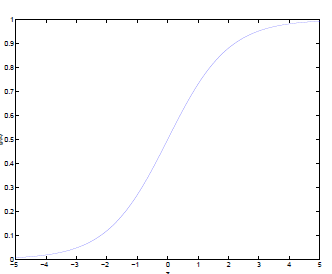
\includegraphics[width=7cm]{fig1}
\end{figure}

可以看到,将无穷映射到了$(0,1)$。

而假设函数就是特征属于$y=1$的概率。
\begin{equation}
P(y=1|x;\theta)=h_\theta(x)
P(y=0|x;\theta)=1-h_\theta(x)
\end{equation}

当我们要判别一个新来的特征属于哪个类时,只需求,若大于$0.5$就是$y=1$的类,反之属于$y=0$类。

再审视一下$h_\theta(x)$,发现$h_\theta(x)$只和$ \theta^T $有关,$\theta^Tx>0$,那么$h_\theta(x)>0.5$,$g(z)$只不过是用来映射,真实的类别决定权还在$\theta^Tx$。还有当时$\theta^Tx>>0$,$h_\theta(x)=1$,反之$h_\theta(x)=0$。如果我们只从$\theta^Tx$出发,希望模型达到的目标无非就是让训练数据中$y=1$的特征$$\theta^Tx>>0$$,而是$y=0$的特征$\theta^Tx<<0$。Logistic回归就是要学习得到$\theta$,使得正例的特征远大于$0$,负例的特征远小于$0$,强调在全部训练实例上达到这个目标。

\subsubsection{形式化标示}
我们这次使用的结果标签是$y=-1$,$y=1$,替换在logistic回归中使用的$y=0$和$y=1$。同时将$\theta$替换成$w$和$b$。以前的$\theta^Tx=\theta_0+\theta_1x_1+\theta_2x_2+\cdots+\theta_nx_n$,其中认为$x_0=1$。现在我们替换为$b$,后面替换$\theta_1x_1+\theta_2x_2+\cdots+\theta_nx_n$为$w_1x_1+w_2x_2+\cdots+w_nx_n$(即$x^Tx$)。这样,我们让$\theta^Tx=w^Tx+b$,进一步$h_\theta(x)=g(\theta^Tx)=g(w^Tx+b)$。也就是说除了$y$由$y=0$变为$y=-1$,只是标记不同外,与logistic回归的形式化表示没区别。

再明确下假设函数
\begin{equation}
h_{w,b}=g(w^Tx+b)
\end{equation}

上面提到过我们只需考虑$\theta^Tx$的正负问题,而不用关心$g(z)$,因此我们这里将$g(z)$做一个简化,将其简单映射到$y=-1$和$y=1$上。映射关系如下:

\begin{equation}
g(z)=\left\{\begin{array}{lr}
1, &z\geqslant0\\
-1, &z<0
\end{array}\right.
\end{equation}

于此,想必已经解释明白了为何线性分类的标准一般用$1$ 或者$-1$ 来标示。

注:上小节来自jerrylead所作的斯坦福机器学习课程的笔记。

\subsection{线性分类的一个例子}
下面举个简单的例子,一个二维平面(一个超平面,在二维空间中的例子就是一条直线),如下图所示,平面上有两种不同的点,分别用两种不同的颜色表示,一种为红颜色的点,另一种则为蓝颜色的点,红颜色的线表示一个可行的超平面。
\begin{figure}[H]
\centering
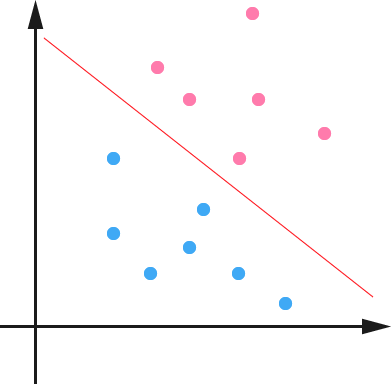
\includegraphics[width=6cm]{fig2}
\end{figure}

从上图中我们可以看出,这条红颜色的线把红颜色的点和蓝颜色的点分开来了。而这条红颜色的线就是我们上面所说的超平面,也就是说,这个所谓的超平面的的确确便把这两种不同颜色的数据点分隔开来,在超平面一边的数据点所对应的 $y$全是 $-1$ ,而在另一边全是 $1$ 。

接着,我们可以令分类函数(提醒:下文很大篇幅都在讨论着这个分类函数):

\begin{equation}
f(x)=w^Tx+b
\end{equation}

显然,如果 $f(x)=0$ ,那么 $x$ 是位于超平面上的点。我们不妨要求对于所有满足 $f(x)<0$ 的点,其对应的 $y$ 等于 $-1$ ,而 $f(x)>0$ 则对应 $y=1$ 的数据点。

\begin{figure}[H]
\centering
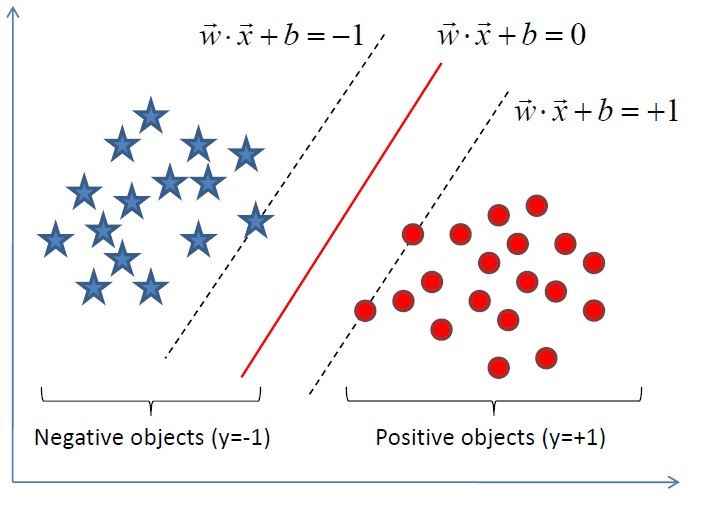
\includegraphics[width=6cm]{fig3}
\end{figure}

注:上图中,定义特征到结果的输出函数$u=\vec w \cdot \vec x -b$,与我们之前定义的$f(x)=w^Tx+b$实质是一样的。为什么?因为无论是$u=\vec w \cdot \vec x -b$,还是$f(x)=w^Tx+b$,不影响最终优化结果。下文你将看到,当我们转化到优化$\max\frac{1}{\|w\|},s.t.,y_i(w^Tx_i+b)\geq1,i=1,\cdots ,n$的时候,为了求解方便,会把$yf(x)$令为$1$,即$yf(x)$是$y(w^x + b)$,还是$y(w^x - b)$,对我们要优化的式子$\max\frac{1}{\|w\|}$已无影响。

(有一朋友飞狗来自Mare Desiderii,看了上面的定义之后,问道:请教一下SVM functional margin 为$ \widehat{\gamma}=y(wTx+b)=yf(x)$中的$\gamma$
是只取$1$和$-1$ 吗?$y$的唯一作用就是确保functional margin的非负性?真是这样的么?当然不是,详情请见本文评论下第43楼)

当然,有些时候,或者说大部分时候数据并不是线性可分的,这个时候满足这样条件的超平面就根本不存在(不过关于如何处理这样的问题我们后面会讲),这里先从最简单的情形开始推导,就假设数据都是线性可分的,亦即这样的超平面是存在的。
    
更进一步,我们在进行分类的时候,将数据点 $x$代入 $f(x)$ 中,如果得到的结果小于 $0$ ,则赋予其类别$ -1$ ,如果大于 $0$ 则赋予类别 $1$ 。如果 $f(x)=0$,则很难办了,分到哪一类都不是。

请读者注意,下面的篇幅将按下述3点走:
\begin{enumerate}
\item 咱们就要确定上述分类函数$f(x) = w\cdot x + b$($w\cdot x$表示w与x的内积)中的两个参数$w$和$b$,通俗理解的话$w$是法向量,$b$是截距(再次说明:定义特征到结果的输出函数$u=\vert w\cdot \vert x-b$,与我们最开始定义的$f(x)=w^Tx+b$实质是一样的);
\item 那如何确定$w$和$b$呢?答案是寻找两条边界端或极端划分直线中间的最大间隔(之所以要寻最大间隔是为了能更好的划分不同类的点,下文你将看到:为寻最大间隔,导出$1/2||w||^2!!!!!!!!!!!!!!!!!!!!!$,继而引入拉格朗日函数和对偶变量$a$,化为对单一因数对偶变量$a$的求解,当然,这是后话),从而确定最终的最大间隔分类超平面hyper plane和分类函数;
\item 进而把寻求分类函数$f(x) = w\cdot x + b$的问题转化为对$w$,$b$的最优化问题,最终化为对偶因子的求解。
\end{enumerate}

总结成一句话即是:从最大间隔出发(目的本就是为了确定法向量$w$),转化为求对变量$w$和$b$的凸二次规划问题。亦或如下图所示(有点需要注意,如读者@酱爆小八爪所说:从最大分类间隔开始,就一直是凸优化问题):
\begin{figure}[H]
\centering

\includegraphics[width=13cm]{fig4}
\end{figure}

\subsection{函数间隔Functional margin与几何间隔Geometrical margin }

一般而言,一个点距离超平面的远近可以表示为分类预测的确信或准确程度。

\begin{itemize}
\item 在超平面$w*x+b=0$确定的情况下,$|w*x+b|$能够相对的表示点x到距离超平面的远近,而$w*x+b$的符号与类标记$y$的符号是否一致表示分类是否正确,所以,可以用量$y*(w*x+b)$的正负性来判定或表示分类的正确性和确信度。
\end{itemize}
于此,我们便引出了定义样本到分类间隔距离的函数间隔functional margin的概念。

\subsubsection{函数间隔Functional margin}
我们定义函数间隔functional margin 为: 

\begin{equation}
\widehat{\gamma}=y(w^Tx+b)=yf(x)
\end{equation}

接着,我们定义超平面$(w,b)$关于训练数据集T的函数间隔为超平面$(w,b)$关于T中所有样本点$(x_i,y_i)$的函数间隔最小值,其中,$x$是特征,$y$是结果标签,$i$表示第$i$个样本,有:
\begin{equation}
\widehat{\gamma}=\min\widehat{\gamma}_i(i=1,\cdots,n)
\end{equation}

然与此同时,问题就出来了。上述定义的函数间隔虽然可以表示分类预测的正确性和确信度,但在选择分类超平面时,只有函数间隔还远远不够,因为如果成比例的改变$w$和$b$,如将他们改变为$2w$和$2b$,虽然此时超平面没有改变,但函数间隔的值$f(x)$却变成了原来的$2$倍。

其实,我们可以对法向量w加些约束条件,使其表面上看起来规范化,如此,我们很快又将引出真正定义点到超平面的距离--几何间隔geometrical margin的概念(很快你将看到,几何间隔就是函数间隔除以个$\|w\|$,即$yf(x) / \|w\|$)。


%\section{公式?!}
%\$ Equation \$ = $ Equation $
%
%\href{http://www.sciweavers.org/free-online-latex-equation-editor}{手点}
%
%
%\href{}{手写}
%
数字与普通运算符号可直接由键盘上键入。下列符号可以直接由键盘键入:

        \begin{center}
                    + \;-\; =\; $<$\; $>$ \;/ \;:\; !\; | \;[\; ] \;(\; )\\
        \end{center}
		
要注意的是, 左右大括号$\{$ $\}$ 在 \LaTeX\ 中有特殊用途。欲排版左大括号, 指令为 $\backslash \{$ ,
右大括号之指令为 $\backslash \}$ 。排版展示数式有以下四种方法可以达到目的:
        \begin{center}
$\backslash$begin$\{$equation$\}$ ... $\backslash$end$\{$equation$\}$\\
$\backslash$begin$\{$displaymath$\}$ ... $\backslash$end$\{$displaymath$\}$\\
$\backslash$[ ... $\backslash$]\\
\$\$ ... \$\$
        \end{center}
除第一种方式外,其余将不对数学式子进行编号。数式内若要排版文字时,必须置于
$\backslash$mbox 指令内,否则将被视为数学符号,譬如,

$$f(x)=x^2-3x+1 \mbox{, where} -2 \leq x \leq 2$$
\section{常见的数学式}
本节列举一些常见的数学式作为练习与未来使用的参考,每个函数都有其特别之处,请仔细观察研究。
读者可以依此为基础,在往后的写作过程中,逐渐累积更多有特殊型态的或符号的数学式,
只要这里出现过的,参照原使档一定写得出来。

\subsection{函数}
    \begin{lstlisting}[language=TeX,numbers=none,frame=lrtb,keywords={begin},label=Binomial,caption=Binomial] 
  $f(x)={n\choose x}p^x(1-p)^{1-x}, \;\; x=0,1,2,\cdots,n$ 
  \end{lstlisting}
  $f(x)={n\choose x}p^x(1-p)^{1-x}, \;\; x=0,1,2,\cdots,n$ 
   
  \begin{lstlisting}[language=TeX,numbers=none,frame=lrtb,keywords={begin},label=Poisson,caption=Poisson] 
  $f(x)=\frac{e^{-\lambda}\lambda^x}{x!}, \;\;  x=0,1,2,\cdots$ 
  \end{lstlisting}
  $f(x)=\frac{e^{-\lambda}\lambda^x}{x!}, \;\;  x=0,1,2,\cdots$
  
  \begin{lstlisting}[language=TeX,numbers=none,frame=lrtb,keywords={begin},label=Gamma,caption=Gamma] 
  $f(x)=\frac{1}{\Gamma(\alpha)\beta^\alpha}x^{\alpha-1} e^{-\frac{x}{\beta}}, \;\; x\geq 0$
  \end{lstlisting}
  $f(x)=\frac{1}{\Gamma(\alpha)\beta^\alpha}x^{\alpha-1}e^{-\frac{x}{\beta}}, \;\; x\geq 0$ 
  
  \begin{lstlisting}[language=TeX,numbers=none,frame=lrtb,keywords={begin},label=Normal,caption=Normal] 
  $f(x)=\frac{1}{\sigma\sqrt{2\pi}}e^{-\frac{(x-\mu)^2}{2\sigma^2}}, \;\;  -\infty < x < \infty $
  \end{lstlisting}
  $f(x)=\frac{1}{\sigma\sqrt{2\pi}}e^{-\frac{(x-\mu)^2}{2\sigma^2}}, \;\;  -\infty < x < \infty $
  
    \begin{lstlisting}[language=TeX,numbers=none,frame=lrtb,keywords={begin},label=Int,caption=\song 积分式与方程式编号] 
  \begin{equation}\label{gamma}%..........label后的名称自订,代表该方程式
  \int^\infty_0 x^{\alpha-1}e^{-\lambda x} dx = \frac{\Gamma(\alpha)}{\lambda^{\alpha}}
  \end{equation}
  \end{lstlisting}
  \begin{equation}\label{gamma}%.................label后的名称自订,代表该方程式
  \int^\infty_0 x^{\alpha-1}e^{-\lambda x} dx = \frac{\Gamma(\alpha)}{\lambda^{\alpha}}
  \end{equation}
  
  方程式 (\ref{gamma})是广义 $\Gamma$ 积分。\footnote{\song这里利用方程式标签(label)来引用方程式,编号将自动更新。}
  
  \begin{lstlisting}[language=TeX,numbers=none,frame=lrtb,keywords={begin},label=Sqrt,caption=\song 开根号] 
  $$f(x)=\sqrt[3]{\frac {\displaystyle 4-x^{3}}{\displaystyle 1+x^{2}}}$$
  \end{lstlisting}
  $$f(x)=\sqrt[3]{\frac {\displaystyle 4-x^{3}}{\displaystyle 1+x^{2}}}$$
  
  \begin{lstlisting}[language=TeX,numbers=none,frame=lrtb,keywords={begin},label=limit,caption=\song 微分与极限(注意大刮号的使用)] 
  $$f'(x)=\frac{df(x)}{dx}=\lim_{h\rightarrow 0} \left( \frac{f(x+h)-f(x)}{h} \right)$$
  \end{lstlisting}  
  $$f'(x)=\frac{df(x)}{dx}=\lim_{h\rightarrow 0}\left(\frac{f(x+h)-f(x)}{h}\right)$$
  
    \begin{lstlisting}[language=TeX,numbers=none,frame=lrtb,keywords={begin},label=upanddown,caption=\song 上下限的使用] 
 $$\int_a^b f(x) dx \approx \lim_{n\rightarrow \infty}\sum_{k=1}^n f(x_k)\triangle x_k$$
  \end{lstlisting} 
  $$\int_a^b f(x) dx \approx \lim_{n\rightarrow \infty}\sum_{k=1}^n f(x_k)\triangle x_k$$
  
  \begin{lstlisting}[language=TeX,numbers=none,frame=lrtb,keywords={begin},label=bast,caption=\song 最佳化问题] 
   $$\max_{\mathbf{u},\mathbf{u}^T\mathbf{u}=1} \mathbf{u}^T\Sigma_X\mathbf{u}$$
  \end{lstlisting} 
  $$\max_{\mathbf{u},\mathbf{u}^T\mathbf{u}=1} \mathbf{u}^T\Sigma_X\mathbf{u}$$
  
  \begin{lstlisting}[language=TeX,numbers=none,frame=lrtb,keywords={begin},label=somesymbles,caption=\song 几个符号]
  $$\mathbf{e}=\mathbf{x}-\mathbf{x}_q=(I-P)\mathbf{x} \in V^{\perp}, \mbox{where}\; V\oplus V^{\perp}=R^p $$
  \end{lstlisting} 
  $$\mathbf{e}=\mathbf{x}-\mathbf{x}_q=(I-P)\mathbf{x} \in V^{\perp}, \mbox{where}\; V\oplus V^{\perp}=R^p $$


\subsection{矩阵与行列式}
矩阵或有规则排列的数学式或组合很常见,以下列举几种模式,请特别注意其使用的标签及一些需要注意的小地方。譬如,
\begin{enumerate}%[a)]
\item 矩阵的左右括号需各别加上。
\item 横行各项之间是以 $\&$ 区隔。
\item 除最后一行外,每行之末则加上换行指令$\backslash$ $\backslash$。
\item 使用array指令时,须加上选项以控制每一直栏内各数字或符号要居中排列、靠左或靠右。
\end{enumerate}
范例与注意事项:
\begin{enumerate}
  \item 左右方框刮号的使用及各直栏的对齐方式:
        $$ A = \left[
            \begin{array}{clr}
                a+b & mnop  & xy \\
                a+b & pn    & yz \\
                b+c & mp    & xyz
            \end{array} \right] $$
\begin{lstlisting}[language=TeX,numbers=none,frame=lrtb,keywords={begin}]
						$$ A = \left[
						\begin{array}{clr}
							a+b & mnop  & xy \\
							a+b & pn    & yz \\
							b+c & mp    & xyz
						\end{array} \right] $$
\end{lstlisting} 

  \item 左右圆框刮号的使用及各式点状:
        $$ A=\left(
            \begin{array}{cccc}
                a_{11} & a_{12} & \cdots & a_{1n}\\
                a_{21} & a_{22} & \cdots & a_{2n}\\
                \vdots & \vdots & \ddots & \vdots\\
                a_{n1} & a_{n2} & \cdots & a_{nn}
            \end{array} \right) $$
\begin{lstlisting}[language=TeX,numbers=none,frame=lrtb,keywords={begin}]
				$$ A=\left(
				\begin{array}{cccc}
					a_{11} & a_{12} & \cdots & a_{1n}\\
					a_{21} & a_{22} & \cdots & a_{2n}\\
					\vdots & \vdots & \ddots & \vdots\\
					a_{n1} & a_{n2} & \cdots & a_{nn}
				\end{array} \right) $$
\end{lstlisting} 

  \item 排列整齐的符号:
        $$ \begin{array}{clr}\\
            a+b+c   & m+n & xy \\
            a+b     & p+n & yz \\
            b+c     & m-n & xz
        \end{array} $$
\begin{lstlisting}[language=TeX,numbers=none,frame=lrtb,keywords={begin}]
					$$ \begin{array}{clr}\\
						a+b+c   & m+n & xy \\
						a+b     & p+n & yz \\
						b+c     & m-n & xz
					\end{array} $$
\end{lstlisting}

    \item 等号对齐的函数组合(不编号)
        \begin{eqnarray*}
          b_1 &=& d_1+c_1 \\
          a_2 &=& c_2+e_2
        \end{eqnarray*}
\begin{lstlisting}[language=TeX,numbers=none,frame=lrtb,keywords={begin}]
						\begin{eqnarray*}
						  b_1 &=& d_1+c_1 \\
						  a_2 &=& c_2+e_2
						\end{eqnarray*}
\end{lstlisting}

    \item 等号对齐的函数组合(编号在最后一行)
        \begin{eqnarray}
\nonumber b_1 &=& d_1+c_1 \\
          a_2 &=& c_2+e_2
        \end{eqnarray}
\begin{lstlisting}[language=TeX,numbers=none,frame=lrtb,keywords={begin}]
					\begin{eqnarray}
						\nonumber b_1 &=& d_1+c_1 \\
						a_2 &=& c_2+e_2
					\end{eqnarray}
\end{lstlisting}

    \item 使用巨集 amsmath 的指令 align(控制编号在第一行)
        \begin{align}
            b_1 &= d_1+c_1\\
            a_2 &= c_2+e_2 \notag
        \end{align}
\begin{lstlisting}[language=TeX,numbers=none,frame=lrtb,keywords={begin}]
					\begin{align}
						b_1 &= d_1+c_1\\
						a_2 &= c_2+e_2 \notag
					\end{align}
\end{lstlisting}

    \item 两组数学式分别对齐
    \begin{align}
        \alpha_1 &= \beta_1+\gamma_1+\delta_1, &a_1 &= b_1+c_1\\
        \alpha_2 &= \beta_2+\gamma_2+\delta_2, &a_2 &= b_2+c_2
    \end{align}
\begin{lstlisting}[language=TeX,numbers=none,frame=lrtb,keywords={begin}]
		\begin{align}
			\alpha_1 &= \beta_1+\gamma_1+\delta_1, &a_1 &= b_1+c_1\\
			\alpha_2 &= \beta_2+\gamma_2+\delta_2, &a_2 &= b_2+c_2
		\end{align}
\end{lstlisting}

    \item 编号在中间(split指令环境)
        \begin{equation}
            \begin{split}
                \alpha_1 &= \beta_1+\gamma_1\\
                \alpha_2 &= \beta_2+\gamma_2
            \end{split}
        \end{equation}
\begin{lstlisting}[language=TeX,numbers=none,frame=lrtb,keywords={begin}]
				\begin{equation}
					\begin{split}
						\alpha_1 &= \beta_1+\gamma_1\\
						\alpha_2 &= \beta_2+\gamma_2
					\end{split}
				\end{equation}
\end{lstlisting}

    \item 只是居中对齐的数学式组(gather指令环境)
        \begin{gather}
        \alpha_1 + \beta_1\notag\\
        \alpha_2 + \beta_2 + \gamma_2\notag
        \end{gather}
\begin{lstlisting}[language=TeX,numbers=none,frame=lrtb,keywords={begin}]
				\begin{gather}
					\alpha_1 + \beta_1\notag\\
					\alpha_2 + \beta_2 + \gamma_2\notag
				\end{gather}
\end{lstlisting}

    \item 长数学式的表达(注意第二行加号的位置)
        \begin{align}
            y   &= x_1 + x_2 + x_3 \notag\\
                &\quad + x_4 + x_5
        \end{align}
\begin{lstlisting}[language=TeX,numbers=none,frame=lrtb,keywords={begin}]
				\begin{align}
					y   &= x_1 + x_2 + x_3 \notag\\
						&\quad + x_4 + x_5
				\end{align}
\end{lstlisting}
\end{enumerate}


\subsection{其他}

  $$X_{n} \stackrel{d}{\longrightarrow} X$$\\
\begin{lstlisting}[language=TeX,numbers=none,frame=lrtb,keywords={begin}]
			$$X_{n} \stackrel{d}{\longrightarrow} X$$
\end{lstlisting}

  $$\overbrace{X_{1} + \ldots + \underbrace{X_{15} + \ldots + X_{30}}}$$\\
\begin{lstlisting}[language=TeX,numbers=none,frame=lrtb,keywords={begin}]
$$\overbrace{X_{1} + \ldots + \underbrace{X_{15} + \ldots + X_{30}}}$$
\end{lstlisting}

  \begin{equation*}
    G = \left\{\begin{array}{l}
          CLASS\#1 \;\;\mbox{if} \;\; \hat{\beta}^T\bf{x} \leq 0 \\
          CLASS\#2 \;\;\mbox{if} \;\; \hat{\beta}^T\bf{x} > 0
        \end{array}\right.
  \end{equation*}\\
\begin{lstlisting}[language=TeX,numbers=none,frame=lrtb,keywords={begin}]
  \begin{equation*}
    G = \left\{\begin{array}{l}
          CLASS\#1 \;\;\mbox{if} \;\; \hat{\beta}^T\bf{x} \leq 0 \\
          CLASS\#2 \;\;\mbox{if} \;\; \hat{\beta}^T\bf{x} > 0
        \end{array}\right.
  \end{equation*}
\end{lstlisting}

以equation或align排版时,数学式会自动编上号码。文稿其他地方若要引述某数学式,
可先以$\backslash$label指令加上标签,再使用$\backslash$ref指令引述。
如此一来若排版文稿须反覆修改,使用$\backslash$label 与$\backslash$ref 指令可以「自动对焦」不会出错。

%
%
%
%\section{图表}
%\subsection{插图}
%
%\begin{figure}[H]
%\includegraphics[width=8cm]{figure1.jpg}
%\caption{Shubert Function}
%\end{figure}
%
%\begin{lstlisting}[language=TeX,numbers=none,frame=lrtb,keywords={begin},label=Gamma,caption=Gamma]
%\begin{figure}[H]
%\includegraphics[width=8cm]{figure1.jpg}
%\caption{Shubert Function}
%\end{figure}
%\end{lstlisting}
%
%\begin{figure}[H]
%\centering
%\includegraphics[width=8cm]{figure1.jpg}
%\caption{Shubert Function}
%\end{figure}
%
%\begin{lstlisting}[language=TeX,numbers=none,frame=lrtb,keywords={begin},label=Gamma,caption=Gamma]
%\begin{figure}[H]
%\centering
%\includegraphics[width=8cm]{figure1.jpg}
%\caption{Shubert Function}
%\end{figure}
%\end{lstlisting}
%\begin{lstlisting}[language=TeX,numbers=none,frame=lrtb,keywords={begin},label=Gamma,caption=Gamma]
%\begin{figure}[H]
%	\begin{center}
%	\includegraphics[width=8cm]{figure1.jpg}
%	\caption{Shubert Function}
%	\end{center}
%\end{figure}
%\end{lstlisting}
%
%
%\begin{figure}[H]
%\centering
%\subfigure[恩恩]{
%\includegraphics[width=4cm]{figure1.jpg}
%\includegraphics[width=4cm]{figure21.jpg}
%}
%\subfigure[呵呵]{
%\includegraphics[width=4cm]{figure1.jpg}
%\includegraphics[width=4cm]{figure1.jpg}
%}
%\caption{The trace of NO.2 player , NO.5 player and ball from cycle 238 to cycle 258}
%\end{figure}
%
%\begin{lstlisting}[language=TeX,numbers=none,frame=lrtb,keywords={begin},label=Gamma,caption=Gamma]
%\begin{figure}[H]
%\centering
%\subfigure[ 恩恩]{
%\includegraphics[width=4cm]{figure1.jpg}
%\includegraphics[width=4cm]{figure21.jpg}
%}
%\subfigure[ 呵呵]{
%\includegraphics[width=4cm]{figure1.jpg}
%\includegraphics[width=4cm]{figure1.jpg}
%}
%\caption{The trace of NO.2 player , NO.5 player and ball from cycle 238 to cycle 258}
%\end{figure}
%\end{lstlisting}
%
%\begin{figure}[H]
%\centering
%\subfigure[the first subfigure]{
%\begin{minipage}[b]{0.2\textwidth}
%\includegraphics[width=1\textwidth]{figure1} \\
%\includegraphics[width=1\textwidth]{figure21}
%\end{minipage}
%}
%\subfigure[the second subfigure]{
%\begin{minipage}[b]{0.2\textwidth}
%\includegraphics[width=1\textwidth]{figure1} \\
%\includegraphics[width=1\textwidth]{figure1}
%\end{minipage}
%}
%\end{figure}
%
%
%\begin{lstlisting}[language=TeX,numbers=none,frame=lrtb,keywords={begin},label=Gamma,caption=Gamma]
%\begin{figure}[H]
%\centering
%\subfigure[the first subfigure]{
%\begin{minipage}[b]{0.2\textwidth}
%\includegraphics[width=1\textwidth]{figure1} \\
%\includegraphics[width=1\textwidth]{figure21}
%\end{minipage}
%}
%\subfigure[the second subfigure]{
%\begin{minipage}[b]{0.2\textwidth}
%\includegraphics[width=1\textwidth]{figure1} \\
%\includegraphics[width=1\textwidth]{figure1}
%\end{minipage}
%}
%\end{figure}
%\end{lstlisting}
%
%
%\subsection{画表}
%
%
%\begin{table}[H]
%\centering
%\caption{Comparison of algorithm efficiency between AINGA and SIGA}
%\begin{tabular}{c|c|c}
%\hline
%Algorithm & Average steps & Success rate /\%\\\hline
%AINGA & 92 & 100\\\hline
%SIGA & 213 & 60\\\hline
%\end{tabular}
%\end{table}
%
%
%\begin{lstlisting}[language=TeX,numbers=none,frame=lrtb,keywords={begin},label=Gamma,caption=Gamma]
%\begin{table}[H]
%\centering
%\caption{Comparison of algorithm efficiency between AINGA and SIGA}
%\begin{tabular}{c|c|c}
%\hline
%Algorithm & Average steps & Success rate /\%\\\hline
%AINGA & 92 & 100\\\hline
%SIGA & 213 & 60\\\hline
%\end{tabular}
%\end{table}
%\end{lstlisting}
%
%
%
%\begin{table}[H]
%\centering
%\caption{Comparison of tackle success rate between the team based on AINGA and the team based on SGA.}
%\begin{tabular}{c|c|c|c|c}
%\hline
%Team & \tabincell{c}{50\\matches} & \tabincell{c}{100\\matches} & \tabincell{c}{200\\matches} & \tabincell{c}{Success \\rate/\%}  \\ \hline
%AINGA & 89\% & 91\% & 90\% & 90\% \\\hline
%Q-Learning & 84\% & 86\% & 83\% & 84.3\% \\\hline
%\end{tabular}
%\end{table}
%
%\begin{lstlisting}[language=TeX,numbers=none,frame=lrtb,keywords={begin},label=Gamma,caption=Gamma]
%\begin{table}[H]
%\centering
%\caption{Comparison of tackle success rate between the team based on AINGA and the team based on SGA.}
%\begin{tabular}{c|c|c|c|c}
%\hline
%Team & \tabincell{c}{50\\matches} & \tabincell{c}{100\\matches} & \tabincell{c}{200\\matches} & \tabincell{c}{Success \\rate/\%}  \\ \hline
%AINGA & 89\% & 91\% & 90\% & 90\% \\\hline
%Q-Learning & 84\% & 86\% & 83\% & 84.3\% \\\hline
%\end{tabular}
%\end{table}
%\end{lstlisting}
%
%\section{参考文献}
%\begin{lstlisting}[language=TeX,numbers=none,frame=lrtb,keywords={begin},label=Gamma,caption=Gamma]
%@article{name1,
%author = {作者, 多个作者用 and 连接},
%title = {标题},
%journal = {期刊名},
%volume = {卷20},
%number = {页码},
%year = {年份},
%abstract = {摘要, 这个主要是引用的时候自己参考的, 这一行不是必须的}
%}
%
%@book{name2,
%author ="作者",
%year="年份2008",
%title="书名",
%publisher ="出版社名称"
%}
%\end{lstlisting}
%
%最简单的使用方法
%
%
%\begin{lstlisting}[language=TeX,numbers=none,frame=lrtb,keywords={begin},label=Gamma,caption=Gamma]
%\bibitem{CK1}Shing-jun Ren and Hai-de Huang (2001). “A Robot Path
%Planning Algorithm Based On Grid Expansion.” Journal of
%Harbin Institute of Technology. Vol.9,No. 11, pp. 68-72.
%\end{lstlisting}
%
%\begin{thebibliography}{11}
%\bibitem{CK1}Shing-jun Ren and Hai-de Huang (2001). “A Robot Path
%Planning Algorithm Based On Grid Expansion.” Journal of
%Harbin Institute of Technology. Vol.9,No. 11, pp. 68-72.
%\bibitem{CK2} Hong-yan Shi, Chang-zhi Sun et al. (2006). “Chaotic
%Potential Field Method and Application in RobotSoccer
%Game.” Proceedings of the 6th World Congress on
%Intelligent Control andAutomation, Dalian, China, June
%2006.
%
%\end{thebibliography}
\end{document}
